\section{Where the Losses Land}
\label{sec:mechanism}

\subsection{Rates and predetermined equity exposure}

The carry result already contains one cross-sectional ordering: the portfolio loses because the high-rate currencies it buys depreciate relative to the low-rate funding currencies. The bilateral estimates in equation~\eqref{eq:bilateral_state} provide a second ordering. State coefficients become more negative as currencies' predetermined equity-market betas rise.

Australia and New Zealand have average betas of 0.20 and 0.13 and annualized state spot coefficients of $-13.21$ and $-13.28$ percentage points. Japan and Switzerland have betas near zero and imprecise coefficients of 2.35 and $-0.89$. Across all nine currencies, regressing the state coefficient on average beta gives a slope near $-60$ percentage points per beta unit, an intercept of $-0.75$, and $R^2=0.77$. With nine observations and no displayed confidence region for the fitted intercept, this is descriptive evidence of a gradient; it does not show that all global exposure vanishes at zero equity beta.

\begin{figure}[H]
    \centering
    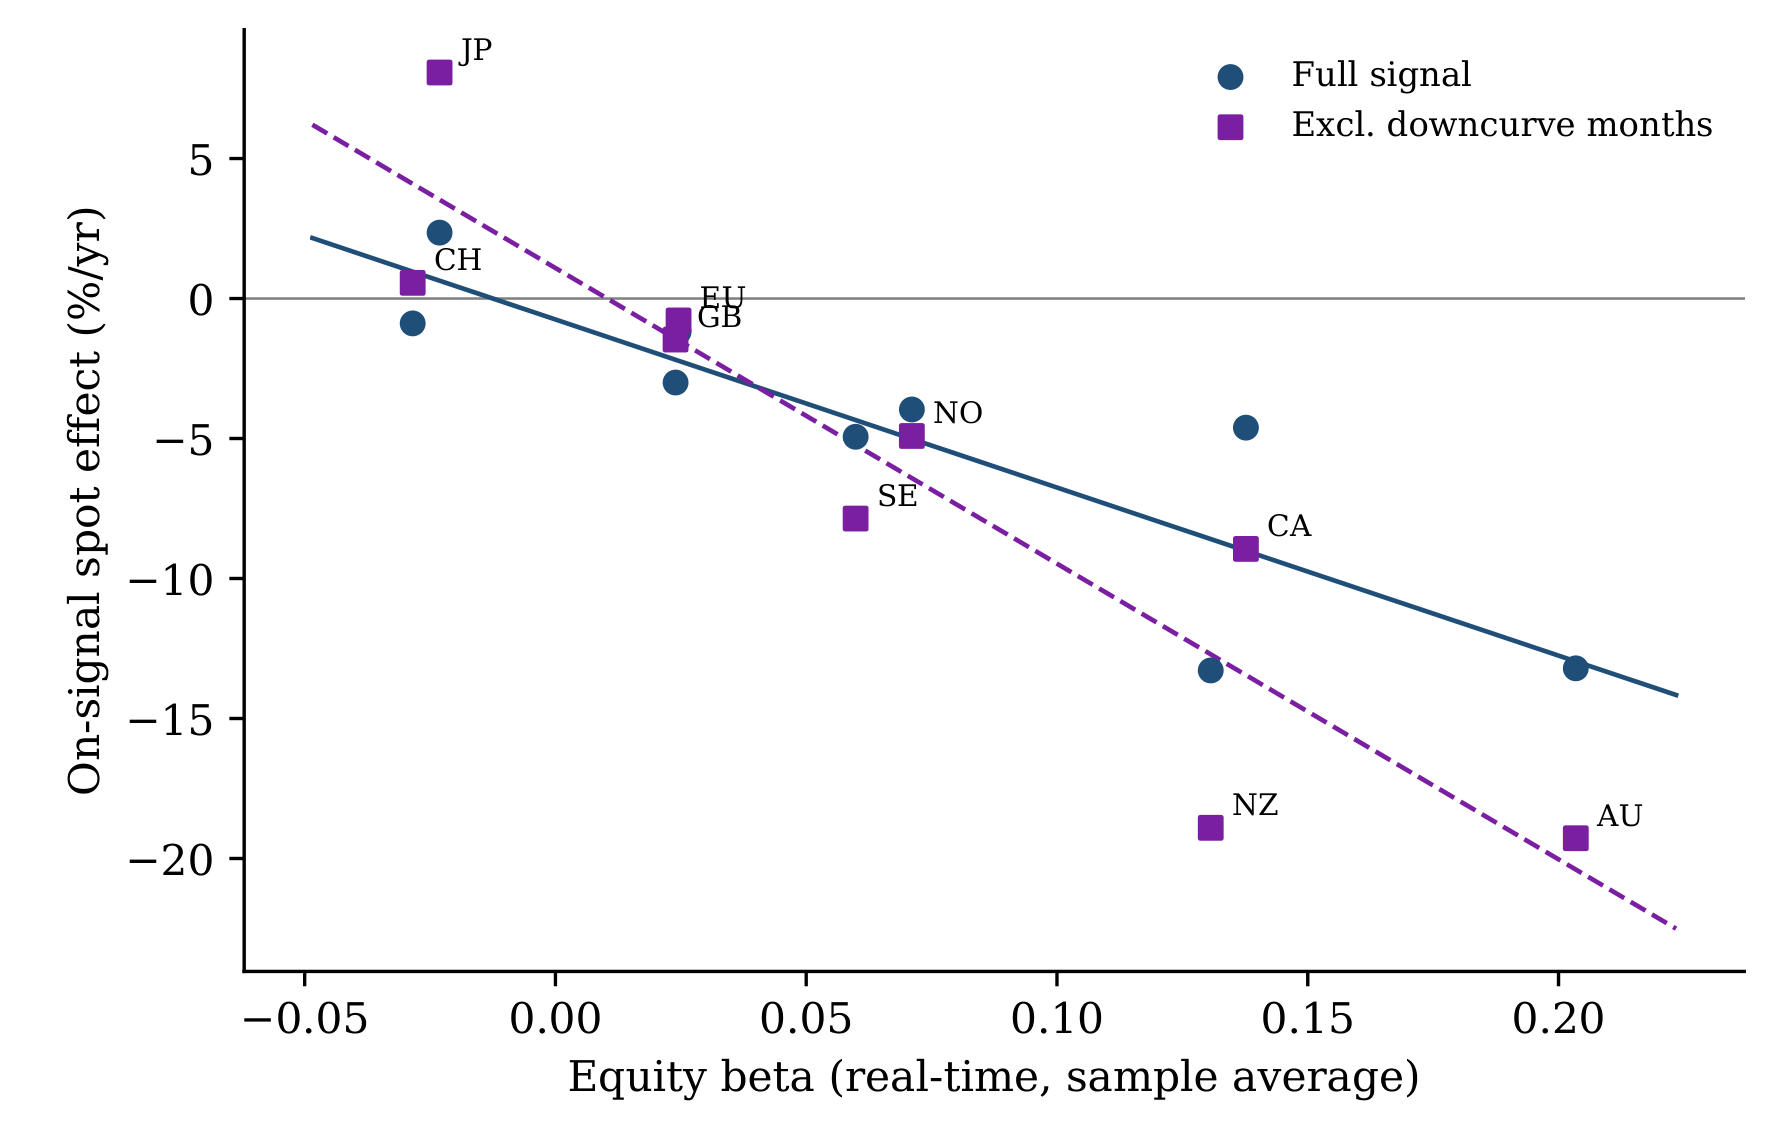
\includegraphics[width=0.94\textwidth]{assets/original/figure_05_main.png}
    \caption{State-dependent spot-return coefficients and predetermined equity beta, one point per currency. Circles and the solid fit show the baseline state (slope $-60$, $R^2=0.77$). Squares and the dashed fit exclude exploratory downcurve months. The baseline inference uses the solid fit.}
    \label{fig:inherited_beta_gradient}
\end{figure}

% SOURCE: AI JMP.pdf pp. 31--36, Table 2, Figure 5, and Table 3. Transcribed, not regenerated.
\begin{table}[H]
\centering
\caption{How active-state losses align with exposure}
\label{tab:exposure-ordering}
\small
\begin{tabularx}{\textwidth}{>{\raggedright\arraybackslash}X r r l}
\toprule
Object & Estimate & Episode wild $p$ & Interpretation \\
\midrule
Rate--beta rank correlation & 0.72 & --- & Descriptive, nine currencies \\
Cross-currency beta slope & $-60$ & --- & Percentage points per beta unit \\
Cross-currency fitted intercept & $-0.75$ & --- & Percentage points at zero beta \\
Cross-currency fit & $R^2=0.77$ & --- & Descriptive, nine currencies \\
Beta-sorted spot portfolio & $-7.53$ & 0.010 & Annualized state difference \\
Panel state $\times$ beta & $-27$ & 0.210 & Annualized interaction \\
Conditional Fama slope, active state & $-1.33$ & 0.340 & $p$-value is for the state interaction \\
\bottomrule
\end{tabularx}

\begin{minipage}{0.94\textwidth}
\footnotesize\emph{Notes:} The cross-currency slope, intercept, and $R^2$ come from regressing the nine bilateral state coefficients on currencies' sample-average predetermined equity betas. The beta-sorted portfolio uses expanding-window betas. The panel interaction uses monthly predetermined betas. The Fama row is supporting conditional-moment evidence; its episode-level uncertainty is wide.
\end{minipage}
\end{table}


The beta-sorted portfolio uses a different predetermined ranking variable but the same underlying currency histories. Its spot return is 7.53 percentage points per year lower in the state, with episode-bootstrap $p=0.010$. The panel interaction between the state and monthly predetermined beta is also negative, about $-27$ percentage points per beta unit, but has $p=0.210$. Thus the carry portfolio establishes the return fact, the beta portfolio supports exposure ordering, the nine-currency scatter is descriptive, and the panel interaction is imprecise.

The high-beta distribution also differs from carry's broad location shift. Its probability of a bottom-decile month rises from 8.5 percent outside the state to 16.3 percent inside ($p=0.046$), while its variance ratio is 1.05 ($p=0.80$). The active state is associated with a higher frequency of adverse returns, not a statistically detectable increase in unconditional variance. The cutoff and several distributional tests were examined jointly, so this remains supporting evidence rather than a separate discovery.

The ordering reflects persistent portfolio membership rather than a wholesale signal-month rotation. New Zealand occupies the carry long leg in 85 percent of all months and 91 percent of active-state months; Australia does so in 71 and 73 percent. Japan and Switzerland remain the core funding currencies. Thus the state primarily reprices standing cross-country exposure rather than changing which currencies the sort holds.

The economics is consistent with several established explanations for persistent currency rankings. Small-country exposure, commodity-export sensitivity, trade-network position, and global intermediary demand can all make high-rate currencies covary more positively with global conditions \citep{hassan2013,ready2017,dellaCorte2016,richmond2019,hassanMano2019,gabaixMaggiori2015}. Common currency factors and business-cycle exposure provide related asset-pricing interpretations \citep{lustigVerdelhan2007,lustig2011,lettau2014,colacito2020}. The rate-beta rank correlation is 0.72 in this sample; it does not establish that one primitive channel generates both rankings.

\subsection{Spot repricing versus predetermined compensation}

Seven floating emerging-market currencies provide a directional out-of-construction check because none enters the G10 state definition. All seven bilateral state coefficients are negative. Pooling them gives annualized spot and total-return effects of $-14.37$ and $-13.35$ percentage points, with episode-bootstrap $p$-values of 0.104 and 0.079. The signs and magnitudes are consistent with a broad international state, but the sample overlaps the G10 episodes and is neither an independent signal replication nor a frozen holdout \citep{bansalDahlquist2000,ilzetzkiReinhartRogoff2019}.

The combined G10-plus-emerging-market carry portfolio isolates the role of compensation. On the common 1996--2026 sample, active-state spot returns are almost identical for G10 carry and G10-plus-emerging-market carry: $-12.79$ and $-12.51$ percent per year. Total returns differ: $-8.67$ for G10 and $+2.51$ for G10 plus emerging markets. The implied active-state income legs are approximately 4.12 and 15.02 percent. The state still lowers the broader portfolio's total return by 9.18 percentage points relative to inactive months, but that estimate is imprecise ($p=0.235$).

This comparison separates two economic objects that the baseline G10 portfolio alone cannot. Synchronized curves locate a similar international spot repricing across the two carry universes; predetermined interest income determines whether that spot loss produces a negative total mean. The state is therefore more naturally interpreted as a spot-risk state than as a universal negative-total-return rule. Online Appendix C reports the common-sample comparison.

\subsection{Supporting conditional moments}

Two additional results are economically coherent but statistically weaker. In a conditional Fama regression, the pooled appreciation slope on the lagged interest differential moves from 0.50 outside the state to $-1.33$ inside it. High-rate currencies therefore depreciate in the active state in point estimates, but the episode-bootstrap $p$-value for the interaction is 0.340. The result is a descriptive regression image of the carry loss, not precise evidence that uncovered interest parity is restored.

The OECD composite leading indicator declines about 0.6 percent over six months after a state month and remains similar around episode onsets and with lag controls. Industrial production also declines in baseline projections but becomes imprecise with the fullest controls. The leading-indicator response is consistent with the yield-curve literature's expected-slowdown interpretation \citep{harvey1988,estrellaHardouvelis1991,estrellaMishkin1998}; the estimates do not establish that synchronized inversions cause activity to fall. Online Appendix C reports the conditional-UIP and local-projection details.

\subsection{A compact compensation benchmark}

A predictable negative conditional return is not implied mechanically by bad-state exposure. The frictionless Euler condition $\E_t[m_{t+1}rx_{t+1}]=0$ says that exposure to high-marginal-utility states should command compensation. To state the timing problem compactly, let an adverse event of size $J>0$ occur at $t+1$ with conditional probability $p_t$. Suppose the known carry income can be written as $C_t=\bar C_t+\mu J\E_{t-1}[p_t]$, where $\bar C_t$ is ordinary carry income and the second term is compensation based on the earlier information set, with $\mu\geq1$. Then
\begin{equation}
    \E_t[rx_{t+1}]
      =\bar C_t+J\bigl(\mu\E_{t-1}[p_t]-p_t\bigr).
    \label{eq:predetermined_compensation}
\end{equation}
A negative conditional mean requires the current perceived loss probability to exceed both previously priced risk and ordinary carry income: $p_t>\mu\E_{t-1}[p_t]+\bar C_t/J$. Fresh synchronized inversions can produce that inequality if bond-market information changes before currency compensation fully adjusts. Slow portfolio adjustment or constrained intermediary capacity are possible frictions \citep{bacchettaWincoop2010,gabaixMaggiori2015}; the reduced-form evidence does not identify either one. Online Appendix B gives the payoff derivation.

\subsection{Alternative common-state interpretations}

Expected-rate news is one candidate. Synchronized curves can reflect coordinated changes in expected policy paths, but lagging the state establishes chronology rather than exogeneity. Common inflation news is another: international yield-curve components contain substantial inflation variation, and disinflation can synchronize inversions without a global growth shock \citep{jotikasthiraLeLundblad2015}. A common term-premium shock is also possible because an inversion is not a pure expectations measure. The asymmetric ACM result---a robust high-beta effect but an attenuated carry effect after the adjustment---keeps that channel open.

Intermediary constraints can jointly affect bonds and exchange rates. Lagged NFCI and VIX do not span the state, but those variables are incomplete proxies for dealer balance sheets, funding conditions, and global risk-bearing capacity \citep{brunnermeier2008,he2017,mirandaRey2020}. Finally, heterogeneous responses to a broad dollar shock can generate some beta ordering even when the average dollar factor is controlled. The evidence makes a uniform one-for-one dollar account less plausible; it does not eliminate every dollar-based mechanism.

The economic conclusion is comparative. The state predicts losses that are ordered by both interest rates and predetermined equity exposure, and the fitted response is small for near-zero-beta currencies. That pattern supports the interpretation that synchronized inversions contain information about a shared international risk rather than only separate national disturbances. It does not identify the primitive shock or the friction that prices it.
